\section{Zufallsvariablen}
Bei einem Zufallsexperiment \wraum\ interessiert man sich oft nicht für das
Ergebnis $\w \in \tO$ sondern für eine Kennzahl $X(\w)$, die von \w\ abhängt.

\paragraph{Beispiel:} n-maliges Würfeln.\\
$\tO  = \{1,2,3,4,5,6\}^n = \{ \w = (\w_1, \dots, \w_n): \w_i \in \{1, \dots, 6\} \; \forall i=1, \dots, n$ \}\\
Mögliche Kennzahlen $X(\w)$ wären:
\begin{align*}
    X(\w) & = \min \w_k \\
    X(\w) & = \max \w_k \\
    X(\w) & = \sum \w_k
\end{align*}

\begin{definition}[Zufallsvariable]
    \label{def:zufallsvar}
    Sei \wraum\ ein W-Raum und $X: \tO \to \real$ eine Abbildung.
    $X$ heißt Zufallsvariable, falls für alle $B \in B(\real)$ gilt:
    \begin{equation*}
        \underbrace{\{\w \in \tO: X(\w) \in B\}}_{\subset \tO} \in \tS
    \end{equation*}
\end{definition}

\paragraph{Bemerkungen}
\begin{enumerate}
    \item Zufallsvariablen sind Abbildungen
    \item Die Aussage aus \autoref{def:zufallsvar} muss hier nicht überprüft
          werden.
          Alle im folgenden auftauchenden Abbildungen sind Zufallsvariablen.
    \item Wir schreiben $\{X \in B\}$ für das Ereignis
          $\{\w \in \tO: X(\w) \in B\}$.
\end{enumerate}

\begin{definition}[Verteilung einer Zufallsvariable]
    Sei $X: \tO \to \real$ eine Zufallsvariable und \wraum\ ein W-Raum.
    Dann heißt das W-Maß $P_X: B(\real) \to [0,1]$ mit
    $P_X(B) = P(\{X \in B\}) = P(\{\w \in \tO: X(\w) \in B\})$, $B \in B(\real)$,
    die \emph{Verteilung} von $X$.
\end{definition}

\todo{Übung: Angeben von Verteilung mit Bsp}

\paragraph{Beachte:}
$X$ bildet den ursprünglichen W-Raum in einen neuen ab:
\begin{center}
    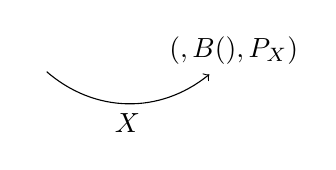
\begin{tikzpicture}
        \node[anchor=south] (a) at (0,0) {\wraum};
        \node[anchor=south] (b) at (2.5,0) {$(\real, B(\real), P_X)$};
        \path[->] (a) edge[bend right=40] node[below]{$X$} (b);
    \end{tikzpicture}
\end{center}

\begin{definition}[Diskrete Zufallsvariablen]
    \begin{enumerate}
        \item Eine Zufallsvariable heißt diskret, falls eine Menge $D \subset \real$
              existiert, die höchstens abzählbar ist mit $P(\{X \in D\})=1$.
        \item Sei $X$ diskret. Die Menge $D_X = \{ x \in \real: P(\{X \in D\})>0 \}$
              heißt der \emph{Träger} von $X$.\\
              Beachte: Es gilt $P(\{X \in D_X \}) = 1$.
    \end{enumerate}
\end{definition}
